\documentclass[output=paper,colorlinks,citecolor=brown,
% hidelinks,
% showindex
]{langscibook}

%This is where you put the authors and their affiliations
\author{Michael Diercks\affiliation{Pomona College}\and Franny Brogan\affiliation{Pomona College}\lastand  Hazel Mitchley\affiliation{Rutgers University}}

%Insert your title here
\title{ACAL Proceedings: Quick Reference Guide for LaTeX}  
\abstract{Here is where you write the abstract of the paper.
}


\input{AcalProceedingsTemplatePackages.tex}
\input{AcalProceedingsTemplateCommands.tex}

\input{localpackages.tex}
\input{localcommands.tex}

% \IfFileExists{../localcommands.tex}{%hack to check whether this is being compiled as part of a collection or standalone
%   \input{../localpackages}
%   \input{../localcommands} 
% \togglepaper[23]
% }{}

\begin{document}
\maketitle

%This just introduces the table of contents for this quick reference guide, and can be deleted if the table of contents is not desired
\begingroup
\let\cleardoublepage\clearpage
\tableofcontents
\endgroup

\section{Introduction}

\textbf{Note}: This document is designed to be read as a \href{https://www.overleaf.com/latex/templates/acal-proceedings-latex-quick-reference-guide/fncrcrtgnxhv}{template on Overleaf}: double clicking on something on the right side of your screen will show you the source code to the left. So you can read the formatted document on the right of the screen, then look to the left to see the code that generated it. If this function stops working, just refresh the webpage.

\LaTeX{} is a typesetting program that takes a text document (with the file type .tex) and converts it to a typeset document that can be easily made into a PDF. \href{https://www.overleaf.com}{Overleaf} is a tool for writing in \LaTeX{}. In Overleaf, the .tex document is in the middle side of your screen; this `code' is \textbf{compiled} to generate typeset document is on the right, which can be downloaded as a PDF by clicking the `Download PDF' icon  at the top of the preview.

When writing a .tex document you directly annotate your text with \textbf{commands} that tell the program how to format the text. So if you want to write something in \textit{italics} you write \verb|\textit{italics}|, and if you want something \textbf{bolded} you write \verb|\textbf{bolded}|. \LaTeX{} then converts that `code' into what looks like italics and bold. In this Overleaf template, you can look at the .tex file itself to see what commands (`code') are used to create different kinds of formatting. 

%In the paragraph above, the command \verb|stuff| is from the package ``verbatim'' which prints whatever is written inside the |vertical lines| even if it is a command that usually does something in LaTeX. Just in case you were wondering what that command is. It's how we get the actual commands themselves to show up in the typeset document to the right.

Double click on this sentence in the preview and see where the cursor moved to in the .tex document to the left of this preview. Then read immediately below this paragraph to see what a ``comment'' is using the \% symbol. 

%As you can see, using the percentage symbol "%" creates a "comment," i.e. something that appears in the .tex document, but which does not compile, and therefore has no effect on the document being produced. It's a handy way to write yourself notes. This does mean that if you ever want to use a % symbol that is NOT for a comment, you have to add a backslash in front of it to tell LaTeX that you don't mean for it to be a comment, like we did in the paragraph above.

%If you want to comment out a bunch of stuff at once in Overleaf, highlight it and Press Cmd-/ (or, Ctrl-/ on a PC). This will but a % in front of every line.

\subsection{What is \LaTeX{} and why am I using it?}

These are very good questions, please check out the \href{https://acal.linguistlist.org/annual-conference-proceedings/}{ACAL website} for more complete answers. The main reason why we write in \LaTeX{} is that it is required by Language Science Press, the press that publishes ACAL proceedings. We discuss why on  \href{https://acal.linguistlist.org/annual-conference-proceedings/}{our website}. A few basic comments are in order, however, so that our explanations below are interpretable. 

Aside from directly annotating text with formatting commands, another difference between apps like Microsoft Word and \LaTeX{} is that \LaTeX{} is more similar to the code that makes Word work, rather than Word itself. \LaTeX{} doesn't come with a user interface, and instead people have created many different sorts of apps to access and use \LaTeX. Overleaf is just one of these apps, which we have chosen for this template because it is convenient in many ways (though it has restrictions too, e.g. requiring internet access).

LaTeX itself has a limited degree of functionality - it does many things, but not all the things. As a result, many people have created packages\textemdash which are essentially plug-ins, or add-ons\textemdash which allow LaTeX to do some extra stuff. Much of the explanations that follow use packages designed by linguists that allow linguists create formatting in their papers that matches their needs: numbered examples, trees, IPA symbols, charts, etc.\footnote{At the very left of your screen, you will see a list of files that make up the \LaTeX{} project. All .tex documents begin with a \textbf{preamble} (the part of the .tex file before the command beginning the document at the top of the text in the .tex file). In this template, we chose to simplify by having the preamble refer to two files that are listed on the left side of your screen: AcalProceedingsTemplatePackages.tex, and AcalProceedingsTemplateCommands.tex. This is where we added the packages we use and the commands we designed for this template (or borrowed from other scholars). You can click on those files to see what things look like in there, but if you are a beginner, we recommend not worrying about that until later.} 

\subsection{What is this document?}

This is a Quick Reference Guide for writing proceedings papers in \LaTeX{} for the \href{https://acal.linguistlist.org}{Annual Conference on African Linguistics}. This guide is published as \href{https://www.overleaf.com/latex/templates/acal-proceedings-latex-quick-reference-guide/fncrcrtgnxhv}{an Overleaf template}. 

\begin{itemize}

\item This guide provides examples of formatting you may need for an ACAL proceedings paper, e.g. trees, numbered examples, etc. 

\item A copy of this project is now in your Overleaf account (i.e. it belongs to you), and you can now edit this document to be an actual paper that you write. This means there is no setup required, you can just erase this text and start typing your own paper, or use this document to practice and see what changes your edits make.\footnote{This also means you will probably want to rename the document - you can do this by hovering your cursor over the title ``ACAL Proceedings Quick Reference Guide' at the top of this page, and then clicking on the pencil icon that appears to the right of the title. You can also rename the AcalProceedingsQuickReference.tex file in the leftmost panel by clicking on the down arrow.} 

\item Designing a \LaTeX{} project from scratch can be difficult; the point of this template is that this is already done for you, you can just start writing. Our \href{https://www.overleaf.com/latex/templates/acal-proceedings-template/kxmngmsjvfqq}{ACAL Proceedings Paper Template} offers the same advantages without this (long) explanatory document.

\item Don't worry about breaking anything - you can always  \href{https://www.overleaf.com/latex/templates/acal-proceedings-latex-quick-reference-guide/fncrcrtgnxhv}{open this template again on Overleaf} to see this initial version again. So edit away!

%Mess with the text in the .tex document right here and see what happens when you Recompile (the green button at the top left of the PDF viewer).

\end{itemize}

\section{Some basic things you will want to know}

For a full \LaTeX{} tutorial, see \href{http://ptmartins.info/latex/}{Pedro Martin's tutorial}. But this section \textit{very} quickly outlines things you may want to know how to do to write ACAL proceedings papers. 

\subsection{Useful commands for text formatting, some that we built for you}
 \label{sec:diercks:UsefulShortcuts}

The chart in \tabref{tab:diercks:CommandsTable} is structured with the most general sorts of text formatting first, with linguistics-specific symbols/formatting at the bottom. Note that the LSP style guide forbids the use of underlining, so do not format anything with underlining. 

\begin{table}
\caption{Selected commands for common ACAL formatting needs}
\label{tab:diercks:CommandsTable}

	\begin{tabular}[t]{l l l}
		\toprule
		\textbf{Symbol/Annotation} & \textbf{Example} & \textbf{Code} \\ \midrule
		Ellipsis & \dots & \verb|\dots| \\
		Underscore & X\textunderscore{}Y & \verb|X\textunderscore{}Y| \\
		Subscript & NP\subs{i} & \verb|NP\subs{i}| \\
		Superscript & NP\supers{i} & \verb|NP\supers{i}|\\ 
		Bold & \textbf{bold} & \verb|\textbf{bold}| \\
		Italic & \textit{italic} & \verb|\textit{italic}| \\
		Small Caps & \textsc{small caps} & \verb|\textsc{small caps}| \\
		Strikeout & \sout{strikeout} & \verb|\sout{strikeout}| \\
		Circle something & \circled{something} & \verb|\circled{something}| \\
		Highlight something & \hl{something} & \verb|\hl{something}| \\
		Null & \nothing  & \verb|\nothing|\\
		Hash & \# & \verb|\#| \\
		Trace with index & \tr{k}  & \verb|\tr{k}| \\
		Bar-level node & X\xbar & \verb|X\xbar| \\
		Head Node & X\xhead & \verb|X\xhead| \\
		Underline & \textit{do not use} & \textit{do not use} \\
		\bottomrule
	\end{tabular}
\end{table}

\begin{itemize}

\item If you want to make a bulleted list, look at how this list is formatted in the .tex document using the ``itemize'' environment. Notice that \verb|\begin{itemize}| starts the bulleted list, \verb|\item| introduces a bullet, and \verb|\end{itemize}| ends the bulleted list.

\item As you've already seen if you are paying attention to the .tex document on the left of your screen, sections, subsections, and sub-subsections are formatted with the commands \verb|\section{}|, \verb|\subsection{}|, and \verb|\subsubsection{}|, respectively.

\item Look at the .tex document to see how we bolded \textbf{this text} (and Overleaf has a shortcut to make it easy, Cmd-B on Macs, Ctrl-B on PCs). \textit{Similarly for italics}, Overleaf provides a shortcut (Cmd-I on Macs, Ctrl-I on PCs).

\item Write footnotes like this.\footnote{Hey, look at me, I'm a footnote.}

\end{itemize}

\subsection{How do I do X?}

You likely will wonder how to do something that seems mysterious in \LaTeX{} but that is so simple in other applications. Google is your friend. Type ``bulleted list in latex" into Google and you will quickly find instructions for a bulleted list, and you can use this method to find out how to do almost anything you need to do. If you still cannot figure out how to solve your \LaTeX{} puzzle, contact the ACAL \LaTeX{} team at \href{mailto:acal.latex@gmail.com}{acal.latex@gmail.com}. 

\subsection{Heads up! Some potential pitfalls}

For all of \LaTeX{}'s conveniences, there are some annoyances that are puzzling until you figure them out. 

\begin{itemize}

    \item Quotation marks are easy to get wrong. You want them to display ``like this'' and not "like this," so use the grave accent symbol above your tab key to type front quotes - use one for a single quote `like this' and two for quotation marks ``like this.'' For reference, the grave accent is the one that appears on the mid vowel here: \`o.

    \item Because a character like the percentage symbol \% actually means something in \LaTeX{} (it creates a comment), you can't just use a percentage symbol on its own to mean a percentage symbol. Instead, you have to put a backslash in front of it, like we did in in the previous sentence (check out the .tex document, and also \href{http://ptmartins.info/latex/#special-characters}{this note} about other similar characters).
    
    \item It is very easy to forget to put the end bracket on a command. So you might write this \verb|\hl{highlight this| instead of \hl{highlight this} (see the .tex) and your document will show an error. Thankfully Overleaf has visual warnings that pop up as you type if you have left a bracket open. (To see this, you can try to highlight something with \verb|\hl{}| in the preceding sentence and leave off the final bracket, Overleaf will highlight text in yellow until the final bracket is added.)
    
    \item Because it's possible to write code that won't compile, it is recommended to compile your document frequently while writing. This way, when you make a mistake you won't have pages and pages to sort through to find where the mistake is. The keystroke Cmd-S (on Mac) and Ctrl-S (on PC) will instruct Overleaf to Recompile, we suggest making it a habit to do this frequently while you write. %This makes things a lot easier, bc trying to find the broken piece of code somewhere inside your whole paper can be a real pain.

\end{itemize}

\section{Numbered examples} \label{sec:diercks:NumberedExs}

It is easy to create consecutively numbered examples: 

%\ea Watch the numbers change when you uncomment this (by deleting the \% symbol) and recompile!  \z 

\ea 
This example is auto-numbered - if you uncomment the example above that is in green in the .tex document (by deleting the \% before the example) and recompile, the numbering will change.
\z 

\noindent The \texttt{gb4e} package that Language Science Press uses for numbered examples allows for inter-linear glossing and translations: 

\ea 
%Language Name \citep{source.citekey.here} \\ %this line is optional
\gll this is a language example \\
this is the morphological gloss \\
\glt `This is the translation.' 
\z 

\noindent  \texttt{gb4e} automatically aligns glosses with the language example (each white space means a different word). This is useful for non-English examples like the Lubukusu sentence in \REF{ex:diercks:BukusuNegation}: 

\ea \label{ex:diercks:BukusuNegation}
%Lubukusu (Justine Sikuku, pc) \\
\gll Wekesa se-a-la-ba a-kula ka-ma-indi ta. \\
Wekesa \Neg-\Sm-\Pst-be \Sm-buy 6-6-maize \Neg{} \\ 
\glt `Wekesa will not be buying maize.'
\z

\noindent Some things to notice in the .tex document for the examples above - an example is started with the \verb|\ea| and ended with \verb|\z| - omitting either of these will generate an error. The language and gloss lines are started with the command \verb|\gll|, with line breaks (\verb|\\|) ending both the language line and the gloss line. The translation line is introduced with the command \verb|\glt|, and notice that there is no line break at the end of the translation line. If you want to label an example as coming from a specific language, Language Science Press places the language name above the example, as is commented out in example \REF{ex:diercks:BukusuNegation}.

If you want multiple data examples to appear in one numbered example, you use the xlist environment to create a sublist, which you can see in the .tex document by double clicking on the example below in the preview: 

\ea \label{ex:diercks:XlistExample}
\begin{xlist}

\ex This is the first example. 

\ex \label{ex:diercks:SwahiliXlist}
\gll hii ni m-fano w-a pili, kwa Ki-swahili \\
this is 3-example 3-\Assoc{} second, of 7-Swahili \\
\glt `This is a second example, in Swahili.' 

\end{xlist}

\z 

\noindent Again, some details to notice in \REF{ex:diercks:XlistExample}: first, notice the commands \verb|\begin{xlist}| and \verb|\end{xlist}| that begin and end the sublist inside the example. It is important that the sublist be generated \textit{inside} the numbered example, so \verb|\begin{xlist}| comes after \verb|\ea| and \verb|\end{xlist}| comes before \verb|\z|. Each example inside the sublist is introduced with the command \verb|\ex|, and each of these examples uses normal gb4e formatting. So you can see that the commands to format \REF{ex:diercks:SwahiliXlist} are the same as were used to generate \REF{ex:diercks:BukusuNegation}.

In many linguistics publications, \textit{all} diagrams and data are presented as numbered examples (e.g. trees, tableaux, charts, sentences with interlinear glosses, data sets of words). However, in Language Science Press trees are generated as figures (see \sectref{sec:diercks:Syntax}, and tables are listed as tables (see \sectref{sec:diercks:BasicTables}). 

Sebastian Nordhoff at Language Science Press has created \href{https://github.com/langsci/guidelines/blob/master/packages/langsci-gb4e/langsci-gb4.pdf}{a helpful detailed document about how to format numbered examples}: if you want/need more detail than we outline here, you can consult that document.

\section{Using cross-references} \label{sec:diercks:CrossReferences}

It is useful to be able to refer your reader to different sections/examples in your paper: for example, we may want to tell you that examples \REF{ex:diercks:BukusuNegation} and \REF{ex:diercks:XlistExample} are built using \texttt{gb4e}, or that if you want to learn about fonts you should read \sectref{sec:diercks:fonts}. There are two components of a cross-reference in text: 

\begin{enumerate}    

\item You must label a particular section or example that you intend to refer to using the command \verb|\label{LabelName}|, where ``LabelName'' has some predetermined portions (according to LSP's style guide) as well as a portion where you use some text description to describe the thing you are labeling: 

\begin{itemize}

\item Section label: \verb|\label{sec:author:yourlabel}|

\item Table label: \verb|\label{tab:author:yourlabel}|

\item Figure label: \verb|\label{fig:author:yourlabel}|

\item Example label: \verb|\label{ex:author:yourlabel}|

\end{itemize}

    
\item You must then use one of these commands to create the cross-reference. 

\begin{itemize}

\item Section reference (will read `\S \#’ in output):\\ \verb|\sectref{sec:author:yourlabel}|

\item Table reference (will read `Table \#’ in output):\\ \verb|\tabref{tab:author:yourlabel}|

\item Figure reference (will read `Figure \#’ in output): \\ \verb|\figref{fig:author:yourlabel}|

\item Example reference with parens — note caps (will read `(\#)’ in output): \\ \verb|\REF{ex:author:yourlabel}| 

\item Example reference without parens — note caps (will read `\#’ in output): \\ \verb|\ref{ex:author:yourlabel}|

\end{itemize}

\item Some examples:\footnote{Look at the .tex on the left to see how to write the commands, and click the hyperlinks in the cross-references to take you to the portion of the document where the label is created.}

\begin{itemize}

\item the Swahili example above can be referenced as \REF{ex:diercks:SwahiliXlist}. If I wanted to refer to it without parentheses, I can use this command: \ref{ex:diercks:SwahiliXlist}.

\item The aforementioned examples occur in \sectref{sec:diercks:NumberedExs}, which describes how to use numbered examples.

\item In \sectref{sec:diercks:Syntax}, \figref{fig:diercks:FirstTree} shows how to draw a syntax tree.

\item  In \sectref{sec:diercks:BasicTables},  \tabref{tab:diercks:SampleTableCenter} shows how to center-align text in cells of a table.

\item These are some selected examples - throughout the entire document you will see these kinds of cross-references being utilized, so you can look at numerous examples if you so wish.

\end{itemize}

\end{enumerate}

Notably, you can only use any of the reference commands (such as the \verb|\REF{LabelName}| command for numbered examples) with labels that already exist somewhere in your paper - attempting to build a cross-reference to a label that does not exist will not stop your document from compiling, but it will result in an additional Yellow Warning from Overleaf next to the Recompile button, and it will result in question marks where the cross-reference ought to be, like this: \REF{ToNothing}. %If you change the reference in the preceding sentence to \REF{ex:diercks:SwahiliXlist} instead of ``ToNothing,'' you should see the Yellow Warnings next to the Recompile button reduce in number by two, and the cross-reference will successfully compile. 

These cross-references are auto-generated every time you compile your document, so as your section/example numbers change as you write your paper, the cross-references update themselves. 

\section{Using IPA symbols} \label{sec:diercks:fonts}

\ea 
ðɪs ɪz haʊ tu raɪt ɪn ʔɑɪpijeɪ. (This is how to write in IPA.)
\z 

\noindent This template is built on Language Science Press's template, which which allows you to enter IPA symbols directly into your .tex document and it appropriately typesets it when creating a PDF. This doesn't tell you how to type the IPA symbols in the first place, though. This requires a non-\LaTeX{} solution.

\begin{itemize}

    \item \textbf{Recommended}: \href{https://scripts.sil.org/cms/scripts/page.php?site_id=nrsi&id=uniipakeyboard}{SIL IPA keyboard} is downloadable on Mac and PC and gives you keystrokes for inserting IPA characters.\footnote{FYI there's no way to type a `\textrhookschwa' via this keyboard (as far as we know), so utilize one of the methods below.}
    
    \item \href{https://www.blugs.com/IPA/}{IPA Palette}
    
    \item \href{https://ipa.typeit.org}{Online IPA keyboard} where you can type symbols and then copy/paste them into your document
    
    \item The web app \href{http://detexify.kirelabs.org/classify.html}{detexify} is a handy tool that allows you to draw the symbol you want and it shows you what packages you need for that symbol, and what commands create it in \LaTeX{}.\footnote{If detexify says ``mathmode" below the command, it means that you should put the command between \$ signs - i.e. \$\backslash your.command\$}
    
    \item The web app \href{https://shapecatcher.com}{shapecatcher} does something similar; you draw the symbol you want and it identifies possible matches and their unicode identifiers.


\end{itemize}

%These are TIPA instructions for those who want them. But I (MJKD) am thinking we can leave this out altogether, bc I think it won't be necessary?? 

% \noindent If you \textbf{do} want a \LaTeX{}-based solution for creating IPA symbols (i.e. if you don't want to use the keyboards above), the \texttt{TIPA} package is the most commonly-used system for processing IPA symbols in \LaTeX{}. (\href{https://www.tug.org/TUGboat/tb17-2/tb51rei.pdf}{This document} is a good resource for the macro names (i.e. commands to draw a symbol) and shortcut characters you'll need if you want to use \texttt{TIPA}.) Crucially, \texttt{TIPA} phonetic symbols can be inputted in the following two ways (look at the .tex document to see how these are coded):
% \begin{enumerate}
%     \item Input macro names in the normal text environment, e.g., \dh\textsci s \textsci z ha\textupsilon\ tu ra\textsci t \textsci n \textglotstop\textscripta pije\textsci.
%     \item Input macro names or \textit{shortcut characters} within the following groups or environment:
%     \begin{itemize}
%         \item \verb|\textipa{...}|, e.g., 
%             \textipa{DIs Iz haU tu raIt In PApijeI}.
%         \item \verb|{\tipaencoding ...}|, e.g., 
%             {\tipaencoding DIs Iz haU tu raIt In PApijeI}.
%         \item \verb|\begin{IPA} ... \end{IPA}|, e.g.,
%             \begin{IPA}
%             DIs Iz haU tu raIt In PApijeI.
%             \end{IPA}
%     \end{itemize}
% \end{enumerate}

% \noindent In our estimation, \texttt{TIPA} is functional if you have to write the occasional IPA character. But the learning curve for \texttt{TIPA} is not much different than the learning curve for the IPA keyboard (and it is harder to read the code in a document coded with \texttt{TIPA}, as you can see in the examples in the list above), so if you are frequently using IPA symbols, you will likely find it easier to learn the IPA keyboard linked to above.


\section{Citing References}

This section is not a proper introduction to all of how citations and bibliographies work in \LaTeX{}. Rather, we attempt to give you the basics you need to know in order to generate citations and a bibliography for an ACAL proceedings paper. 

\subsection{How bibliographies work}

You will notice on the left side of the Overleaf display there is a list of files. The file titled ``localbibliography.bib'' is the bibliography file, and contains references that can be cited in your document. Click on it to see what a \LaTeX{} reference list looks like, and then click on ``AcalProceedingsQuickReference.tex'' to come back here. 

As you write, you can type commands into your text which will do two things: first, they will generate citations in the text to the paper you cite, and second, when your document compiles they will add that reference to your bibliography at the end of your paper. So if you want to make reference to \citet{BresnanMchombo1987ChichewaSmOm}, enter the citation command as we did in the .tex document, which references the file bibliographic entry in ``localbibliography.bib'' and generates the appropriate citation here in this paragraph, and adds the \citeauthor{BresnanMchombo1987ChichewaSmOm} paper to the bibliography/reference list at the end of this document.

The subsections that follow explain in more detail how to do this in your own paper. 

\subsection{Building a bibliography in a .bib file}

There are many ways to build your reference list: we outline two major ones here.\footnote{If you consistently write in \LaTeX{} you eventually would build a large .bib file that you use on every project; our goal in this explanation is mainly to help novices learn enough to write their current paper.}

First, if you have already created bibliographic references, you can use \citet{Nordhoff2018} (which is located \href{http://glottotopia.org/doc2tex/doc2bib}{here}) to convert those references to a format appropriate for \LaTeX{}. You can then copy and paste those references into ``localbibliography.bib'' which makes them available to cite in your paper.

Second, you can download a reference manager, which produces reference lists that look like what you see in ``localbibliography.bib'' but which gives you a user-friendly interface. If you are using a Mac, \href{https://bibdesk.sourceforge.io}{BibDesk} is an excellent application that will manage your citations - a brief introductory video is \href{https://www.youtube.com/watch?v=sOxf1bKAxqQ}{available on Youtube}. If you are using a PC, we recommend using \href{http://www.jabref.org}{Jabref}, which has the same functionality. Those reference managers will allow you to build a .bib file, which can be copied/pasted into ``localbibliography.bib.'' 

\subsection{What is a cite key?}

If you use the \href{http://glottotopia.org/doc2tex/doc2bib}{Bib converter}, you will notice that the first line of a bibliographic entry is auto-generated as ``AuthorDate'' which is ``Bloomfield1925'' in the example below (which is the first example in the \href{http://glottotopia.org/doc2tex/doc2bib}{Bib converter} sample). 

\indent @article\{\circled{Bloomfield1925}, \\
\indent \indent author = {Bloomfield, Leonard}, \\
\indent\indent journal = {Language}, \\
\indent\indent number = {4},\\
\indent\indent pages = {130--156},\\
\indent\indent title = {On the sound-system of central {Algonquian}},\\
\indent\indent volume = {1},\\
\indent\indent year = {1925}\\
\indent\indent\} \\

\noindent This circled text above is the ``cite key,'' which is an identifier that you use to cite that reference (this can in fact be any string of text that you choose).

\subsection{Citing sources}


The two most important citation commands are \verb|\citet{}| and \verb|\citep{}|. The cite key of the reference goes between the curly brackets.
 
 \begin{itemize}
 
 \item For `Author (Date)' format, use \verb|\citet{}|. \\
  e.g.: writing \verb|\citet{Lahiri2000}| produces \citet{Lahiri2000}, because the cite key `Lahiri2000' refers to the associated reference in the localbibliography.bib file you can see in the file structure to the left.
 \item For a parenthetical citation, use \verb|\citep{}|.\\
 e.g.: writing \verb|\citep{Lahiri2000}| produces \citep{Lahiri2000}, again because the cite key `Lahiri2000' refers to the associated reference in the localbibliography.bib file you can see in the file structure to the left.
 
 \end{itemize}

\noindent Both of these commands can be modified to add extra information.
 
 \begin{itemize}
 \item To add a page number after the year, put the page number in square brackets \textit{before} your curly brackets.\\
 e.g.: \verb|\citep[87]{Doke1923}| produces \citep[87]{Doke1923} 
 \item To add information before the citation, put this in square brackets before the brackets with the page number.\\
  e.g.: \verb|\citep[Zulu,][87]{Doke1923}| produces \citep[Zulu,][87]{Doke1923} 
  \item If you want information before the citation, but without a page number, just leave the page number blank.\\ 
  e.g. \verb|\citep[Zulu,][]{Doke1923}| produces \citep[Zulu,][]{Doke1923}
  \item Multiple cite keys separated by commas will produce multiple citations, assuming that you have put references associated with those cite keys into localbibliography.bib.\\
  e.g. \verb|\citep{Doke1923,Lahiri2000}| produces \citep{Doke1923,Lahiri2000}

 \end{itemize}
 

\noindent You can check out this \href{http://merkel.texture.rocks/Latex/natbib.php}{helpful reference sheet} that gives many details about citation commands for any additional variants that you want. %LSP uses biblatex, not natbib, but their template (and this one) are designed so that the natbib commands work. 

\section{Basic tables} \label{sec:diercks:BasicTables}

Tables are very useful for formatting data and examples, but counter-intuitive to produce in \LaTeX{} as compared to producing them in familiar word processors. This section lays out the basics; check out \href{https://en.wikibooks.org/wiki/LaTeX/Tables}{this useful wiki} on how to construct \LaTeX{} tables if you want some addition information, or Overleaf's  \href{https://www.overleaf.com/learn/latex/Tables}{tables tutorial}.

The \texttt{tabular} environment is used to typeset tables. By default, \LaTeX{} tables are drawn without any vertical or horizontal lines and column width is predetermined; this means that any settings beyond these defaults must be defined by you. Per LSP's guidelines, tables should not have vertical borders in ACAL Proceedings papers. Let's take a look at some simple examples below. Please note, tables are moved around by \LaTeX{} in the typeset document on the right of your screen to where they typeset most naturally, so you may have to look to the next page for a table. Also, please pay attention to the commented-out text that appears in green in the .tex document around each table's code, because we have explained what each part of the code for the table does.   %If for some reason you view vertical borders as a necessity, please get in contact with your volume's editors rather than submitting a paper that includes them.


Let's start with a basic 3x3 table with single horizontal borders. Take a look at the .tex doc to see how borders and column alignment are specified (i.e. whether your text is aligned on the left, right, or in the center of the column) for \tabref{tab:diercks:FirstSampleTable} below. 

\begin{table}

\caption{A descriptive caption here}
\label{tab:diercks:FirstSampleTable}

\begin{tabular}{lll} %the three `l's' mean there are three columns, and that they are left-aligned (hence `l'). 
\lsptoprule %This (\lsptoprule) is a required piece of formatting for tables in LSP volumes (and, therefore, in ACAL proceedings volumes) 
cell 1 & cell 2 & cell 3 \\ 
cell 4 & cell 5 & cell 6 \\
cell 7 & cell 8 & cell 9 \\
\lspbottomrule %This (\lspbottomrule) is a required piece of formatting for tables in LSP volumes (and, therefore, in ACAL proceedings volumes) 
\end{tabular}

\end{table}

%Note that the contents of cells in a given row are separated by '&'. You should have the same number of '&' signs in every row, even if the contents of a given cell are blank (i.e. a blank cell will look like this: & &). Also note that new rows are created using '\\'. This is a more general LaTeX command you can use for manually starting a new line.

\tabref{tab:diercks:SampleTableHeaders} is a table that's identical to the one above, but with column headers separated by a double horizontal line. Take a look at the code in the .tex document to see how it's different from the code that generated the table above. %\verb|You can generate as many horizontal lines as you'd like by duplicating the \hline command.| 

\begin{table}

  \caption{This table separates headers with a double line}
  \label{tab:diercks:SampleTableHeaders}
  
\begin{tabular}{lll}
\lsptoprule %This (\lsptoprule) is a required piece of formatting for tables in LSP volumes (and, therefore, in ACAL proceedings volumes) 
Header 1 & Header 2 & Header 3 \\
\midrule\midrule
cell 1 & cell 2 & cell 3 \\
cell 4 & cell 5 & cell 6 \\
cell 7 & cell 8 & cell 9 \\
\lspbottomrule %This (\lspbottomrule) is a required piece of formatting for tables in LSP volumes (and, therefore, in ACAL proceedings volumes) 


\end{tabular}
\end{table}

\noindent Finally, \tabref{tab:diercks:SampleTableCenter} is a table identical to the one above, but with text center-aligned.

\begin{table}

  \caption{This table has center-aligned text}
  \label{tab:diercks:SampleTableCenter}

\begin{tabular}{ccc}
\lsptoprule %This (\lsptoprule) is a required piece of formatting for tables in LSP volumes (and, therefore, in ACAL proceedings volumes) 
Header 1 & Header 2 & Header 3 \\
\midrule\midrule
cell 1 & cell 2 & cell 3 \\
cell 4 & cell 5 & cell 6 \\
cell 7 & cell 8 & cell 9 \\
\lspbottomrule %This (\lspbottomrule) is a required piece of formatting for tables in LSP volumes (and, therefore, in ACAL proceedings volumes) 

\end{tabular}
\end{table}

In general, LSP's style guide disallows both horizontal borders and vertical borders between cells in a table (apart from horizontal border separating the headers from the rest of the cells, which is coded with \verb|\midrule|.

\subsection{If a table runs off the page}

It is not uncommon to generate a table that can't fit straightforwardly on to the page, like table \ref{tab:diercks:toolongtable}. You can fix this by using the \verb|\fittable{}| command, as exemplified in table \ref{tab:diercks:fittablelongtable}. If you look at the .tex document, you'll see that \verb|\fittable{| comes \textit{before} \verb|\begin{tabular}|, and the closing brace \} for this command comes after \verb|\end{tabular}|.

%Another common requirement is fitting a table or other element which is a bit too large on the page. In order to do this, use \fittable{stuff to resize}. This works for figures as well.

\begin{table}
  \caption{This table is too long}
  \label{tab:diercks:toolongtable}
\begin{tabular}{cccc}
\lsptoprule %This (\lsptoprule) is a required piece of formatting for tables in LSP volumes (and, therefore, in ACAL proceedings volumes) 
Header 1 & Header 2 & Header 3 & Header 4\\
\midrule\midrule
Long piece of data 1 & Long piece of data 2 & Long piece of data 3 & Long piece of data 4  \\
Long piece of data 5 & Long piece of data 6 & Long piece of data 7 & Long piece of data 8 \\
\lspbottomrule %This (\lspbottomrule) is a required piece of formatting for tables in LSP volumes (and, therefore, in ACAL proceedings volumes) 
\end{tabular}
\end{table}

\begin{table}
  \caption{Long table with the \backslash fittable command}
  \label{tab:diercks:fittablelongtable}
\fittable{\begin{tabular}{cccc}
\lsptoprule %This (\lsptoprule) is a required piece of formatting for tables in LSP volumes (and, therefore, in ACAL proceedings volumes) 
Header 1 & Header 2 & Header 3 & Header 4 \\
\midrule\midrule
Long piece of data 1 & Long piece of data 2 & Long piece of data 3 & Long piece of data 4  \\
Long piece of data 5 & Long piece of data 6 & Long piece of data 7 & Long piece of data 8 \\
\lspbottomrule %This (\lspbottomrule) is a required piece of formatting for tables in LSP volumes (and, therefore, in ACAL proceedings volumes) 
\end{tabular}}
\end{table}

We don't go into more depth here in order to keep the length of this overview constrained, but \LaTeX{} allows for endless tinkering with the formatting if you need those kinds of adjustments in your paper. For a comprehensive ``how-to'' guide, see Overleaf's fantastic \href{https://www.overleaf.com/learn/latex/Tables}{tables tutorial}. 

\section{Syntax Things} \label{sec:diercks:Syntax}

\subsection{Trees trees trees}

One of the biggest things syntacticians rely on \LaTeX{} for is drawing trees. This template uses the package \texttt{forest}, so to draw a tree in this template you use the \verb|\Forest{tree.in.here}| command.\footnote{It's worth noting that \href{http://ptmartins.info/latex/}{Pedro Martin's tutorial} does not use the \texttt{forest} package, instead using \texttt{qtree}. This means that the commands used to build trees here are different than what he uses in his tutorial.} 

\begin{figure}
\caption{First example of a tree with Forest. Double-click on this to take you to the code in the .tex document to the left.}
  \label{fig:diercks:FirstTree}
\Forest{
[VP [V\xhead] [NP] ] 
} %don't forget the bracket that ends the tree!!
\end{figure}

\noindent The code for trees uses a standard bracketing notation, so every open bracket has to have a corresponding closing bracket later. This also means that you have to be careful not to forget the second curly bracket at the very end of the code for the tree, matching the open bracket that is part of the \verb|\forest{}| command.

% This is sample code designed for easy copy-pasting into another document (or into another spot in this document) to build new trees. 

% \begin{figure}
% \caption{}
%   \label{}
% \Forest{
% [treeP 
%     [basic] 
%     [tree] 
% ] 
% }
% \end{figure}

The code for \figref{fig:diercks:FirstTree} is formatted so that each level is on the same line. This is not necessary; the code for \figref{fig:diercks:FirstTreeExpanded} has the same exact bracket structures, just with line breaks and indents to visually clarify the levels of the trees. You'll see in the preview that these trees are identical, despite the code in the .tex document being formatted differently.

\begin{figure}
\caption{Same tree as \figref{fig:diercks:FirstTree}, with code formatted differently in the .tex document on the left}
  \label{fig:diercks:FirstTreeExpanded}
\Forest{
[VP 
    [V\xhead] 
    [NP] 
] 
}
\end{figure}

\noindent Please format your code something more like  \figref{fig:diercks:FirstTreeExpanded} than \figref{fig:diercks:FirstTree}, largely because as the trees get larger it can get tougher and tougher to interpret your code and editors may need to wrestle with that at some point. We encourage you to try editing the trees above and see what happens! 

An important note: do not include empty lines in the code for the tree - as you can see, if you add an empty line to the trees above and attempt to recompile, you will get an error. \texttt{forest} attempts to parse all lines so empty lines confuse it. But extra white spaces within a line do not make a difference to \texttt{forest}.

In the example below, we've drawn a slightly bigger tree, which includes an empty node (which is created with an open-close bracket sequence with nothing inside it. 

\begin{figure}
\caption{Slightly bigger tree}
  \label{fig:diercks:SlightlyBiggerTree}

\Forest{
[VP
    [] %this is the empty node
    [V\xbar
        [V\xhead]
        [NP]
    ]
] 
}

\end{figure}


You will notice in the tree above that because there is an empty branching node, the branches don't all go at precisely the same angle. There are spacing options you can invoke to adjust this, as in \figref{fig:diercks:ForestNiceEmptyNodes}, where the top node in the tree is specified as having ``nice empty nodes:'' 

\begin{figure}
\caption{Example of ``nice empty nodes''}
  \label{fig:diercks:ForestNiceEmptyNodes}

\Forest{
[VP, nice empty nodes %Notice the change here
    []
    [V\xbar
        [V\xhead]
        [NP]
    ]
] 
}

\end{figure}

\noindent This is really only helpful for a tree where there are empty branching nodes. We suspect many syntacticians will prefer the nice empty nodes option when there are empty nodes ... but it can cause some messes with more complex trees, so there are times when it is advisable to simply live with some slightly off-angle brackets (unless someone is a master \LaTeX{} user, but this document is not for them). 

\noindent If you want to include text under a node, you include a line break (two backslashes) and add the text, as with the verb below. If you want to include a triangle, you include the desired text in square brackets followed by the code ``, roof'' as seen in \figref{fig:diercks:FullVpTree}. (The comma is part of the code, don't leave it out.)

\begin{figure}
\caption{Example with texts in multiple nodes}
  \label{fig:diercks:FullVpTree}
\Forest{
%for tree={s sep=10mm, inner sep=0, l-=3mm}
    [VP 
    [DP [Maya, roof] ] %notice the triangle code here
    [V\xbar 
        [V\xhead \\ kick ] %text added to head here
        [DP [the ball, roof] ] 
    ] 
]
}
\end{figure}

%You'll notice in the code for the tree in (\ref{FullVpTree}) that there are some specific annotation for tree dimensions (sep, inner sep, etc) commented out. See \S \ref{AdvancedForest} for details about how this works. You can also uncomment it and see what happens.

\noindent Some larger tree skeletons are commented out immediately below this paragraph in case you want a template to work from for a larger tree. Remember, to (un)comment batches of text in Overleaf, highlight the text and press Cmd-/ (Mac) or Ctrl-/ (PC). 

% \begin{figure}
% \caption{Sample larger tree}
%   \label{fig:diercks:LargerSkeleton}
% \Forest{
% [CP
%   []
%   [C\xbar
%         [C\xhead]
%         [TP 
%             []
%             [T\xbar 
%                 [T\xhead]
%                 [VP 
%                     []
%                     [V\xbar
%                         [V\xbar]
%                         [NP]
%                     ]
%                 ] 
%             ] 
%         ] 
%     ]
% ]
% }
% \end{figure}


% \begin{figure}
% \caption{Another sample larger tree}
%   \label{fig:diercks:SecondLargerTree}
% \Forest{
% [CP, nice empty nodes
%   []
%   [C\xbar
%         [C\xhead]
%         [TP 
%             []
%             [T\xbar 
%                 [T\xhead]
%                 [VP 
%                     []
%                     [V\xbar
%                         [V\xbar]
%                         [NP]
%                     ]
%                 ] 
%             ] 
%         ] 
%     ]
% ]
% }
%\end{figure}


\noindent A head-final tree is illustrated in \figref{fig:diercks:HeadFinalTree}, where the difference is what you would expect: the node for the head follows the node for the complement of the head. 

\begin{figure}
\caption{Example of head-final tree}
  \label{fig:diercks:HeadFinalTree}
\Forest{
[CP, %nice empty nodes
  []
  [C\xbar
        [TP 
            [DP [subject, roof] ]
            [T\xbar 
                [VP 
                    []
                    [V\xbar
                        [DP [object, roof] ]
                        [V\xhead \\ verb ]
                    ]
                ]
                [T\xhead]
            ] 
        ]
        [C\xhead]
    ]
]
}
\end{figure}

\subsection{Annotating Trees}

\subsubsection{Basic Arrows in Trees}

Arrows are drawn in a tree with the command \verb|\draw|. You must name specific nodes in your tree, and then you can draw an arrow from one node to the other in the last line of code in the tree. In the tree in \figref{fig:diercks:ForestDrawArrows} we named the triangled DP ``SUBJ'' using the command ``, name=SUBJ''and the trace in Spec,VP as ``SpecVP'' using the command ``, name=SpecVP''. (Like for triangles above, the comma is part of the command, so don't leave it out!) We then used those names in the command to draw the arrow, which is the last line of code in the tree. 

\begin{figure}
\caption{Example of arrows in a tree}
  \label{fig:diercks:ForestDrawArrows}
\Forest{
for tree={s sep=10mm, inner sep=0, l-=3mm}
[TP
    [DP\subs{k} [Maya, roof, name=SUBJ] ] %named this node SUBJ
    [T\xbar
        [T\xhead \\ will ]
        [VP 
          [ \tr{k}, name=SpecVP ] %named this node SpecVP
          [V\xbar 
              [V\xhead \\ kick ]
              [DP [the ball, roof] ] 
          ] 
        ] 
    ]
]
\draw[->] (SpecVP) to[out=south west,in=south] (SUBJ); %Draws arrow
}
\end{figure}

%The argument of draw is used to indicate the direction the arrow should be pointing: up [->], or down [<-], both [<->], or none [-]. 

\subsection{Want to get more fancy with your trees?}

There are a host of additional commands and packages you can use to decorate your trees and/or re-arrange the spacing of nodes, branches, etc. We don't go into detail here because this document is aimed at those just starting to use \LaTeX{}. If you have a particular need for your paper with respect to tree-formatting, you can use Google to find a solution, you can read \href{http://mirrors.ibiblio.org/CTAN/info/forest-quickstart/ForestQuickstart.pdf}{Guido Vanden Wyngaerd's quickstart guide} to \texttt{forest} for linguists, or you can email the ACAL \LaTeX{} committee at \href{mailto:acal.latex@gmail.com}{acal.latex@gmail.com}.

\section{Phonology Things} \label{sec:diercks:Phonology}

\subsection{SPE Rules}
Typing up SPE-style rules in Word/Google Docs can be annoying, even if you're using Bruce Hayes's handy `HowToBrackets' guide. Luckily, typesetting phonology rules in \LaTeX{} is relatively straightforward. This template uses the package \texttt{phonrule}, which employs the basic command \verb|\phon{target}{change}| and then builds on that for more complex rule types. 

The command \verb|\phon{target}{change}| has two arguments: the first is the \textbf{target}, or input, of the rule, and the second is the \textbf{change}, or output. Let's say we have a rule that raises /e/ to [i]. Here, `/e/' is our \textbf{target} and `[i]' is our \textbf{change} (double-click on the rule below to see the code for it):

\phon{e}{i}

Now, let's say this rule only applies in a particular \textbf{environment}, or context. We'll need to add an \textbf{environment} to our rule, which we can do by modifying our command and adding a third (and sometimes a fourth) argument. There are three distinct commands you can use when you want to add an environment to your rule; which one you choose depends on \textit{where you want your environment to appear with respect to the place holder line (i.e., underscore)}: \verb|\phonr|, \verb|\phonl|, and \verb|\phonb|.
\begin{itemize}
    \item \verb|\phonl{target}{change}{environment}| will place your environment \textbf{to the left} of your place holder line: \phonl{e}{i}{u}
    \item \verb|\phonr{target}{change}{environment}| will place your environment \textbf{to the right} of your place holder line: \phonr{e}{i}{]\subs{word}}
    \item \verb|\phonb{target}{change}{left environment}{right environment}| will place the two components of your environment \textbf{on either side} of your place holder line: \phonb{e}{i}{u}{\Rb{word}}
\end{itemize}

Now, what if we want to write some or all parts of our rule using \textbf{feature specifications} instead of IPA symbols? The \verb|\phonfeat[]{}| command allows you to insert feature matrices into your rules using the same argument structure we saw above. Let's take a look at an example:

\ea \label{ex:diercks:EngAspRule}
English Aspiration Rule: \\
\phonl{\phonfeat[c]{-voice\\-delayed release}}
{[+spread glottis]}
{\Lb{word}} 
\z

\noindent Keep in mind that you can use the \verb|\phonfeat[]{}| command to insert feature matrices of any size into any part of your rule (the target, change, and/or environment) following the format presented in example \REF{ex:diercks:EngAspRule} above.

As you may know, the English Aspiration Rule in \REF{ex:diercks:EngAspRule} is incomplete; we need to add an additional environment. For rules that have more than one environment, we can add \textbf{curly brackets} to the environment of our rule, by using the command \verb|\oneof{Context 1 \\ Context 2}|. Double click on rule in \REF{ex:diercks:EngAspRule} to check out the code in the .tex document.

\ea \label{ex:diercks:EngAspRuleRev}
English Aspiration Rule (revised): \\ 
\phonc
{\phonfeat[c]{-voice\\-delayed release}}
{[+spread glottis]}
{\oneof[l]{\Lb{word}\phold \\ 
\Lb{\textsigma}\phold \phonfeat{+syllabic \\ +stress}}}
\z

%In the code above, the '\oneof[l]{}' command gives us curly brackets containing left-aligned text. Change the 'l' to 'r' or 'c' to change the text alignment. The `\phold' command manually creates a place holder line.

Click here to see a template of this rule (in the comments of the .tex document) which you can copy-paste into your document to edit.

% Replace the words `target', `change', `Context1',and  'Context2' with  the relevant information. Make sure not to delete any of the curly brackets!
%
%    \phonc{target}{change}{\oneof[l]{Context1 \\ Context2}}.
%
% You can add additional contexts by adding ``\\ [additional context]'' after Context2.




\subsection{Phonemicization diagrams}\label{sec:diercks:PhonDia}
For phonemicization diagrams, this template uses the \texttt{TikZ} package, which is a general tool for creating graphic elements in \LaTeX{}. Once you understand the basic structure of these diagrams, adding additional tiers, changing the information conveyed in your tier(s), and modifying association lines is fairly simple. 

 As you'll see in the .tex document, we're simply creating a series of ``nodes", naming them, positioning them in relation to one another using (x,y) coordinates, and then specifying what text each node should contain. Once each node has been named, we use the \verb|\draw| command to draw association lines between the nodes of our choice. Below are three sets of phonemicization diagrams of varying complexities so you can see how this works:

%You can adjust the (x,y) coordinates below and see the nodes move around, which will help you get a sense of how to control positioning of nodes. Be sure you understand the simple ones before moving to the complex ones.

\ea A simple set of phonemicization diagrams

\begin{tikzpicture}
%phoneme tier
\node (p1) at (1.5,1) {/b/};
\node (p2) at (4.5,1) {/d/};
%allophone tier
\node (a1) at (1,0) {[β]};
\node (a2) at (2,0) {[b]} ;
\node (a3) at (4, 0) {[ð]};
\node (a4) at (5, 0) {[d]} ;
%association lines
\draw (p1) -- (a1);
\draw (p1) -- (a2);
\draw (p2) -- (a3);
\draw (p2) -- (a4);
\end{tikzpicture}
\z

\ea A slightly more complex set of phonemicization diagram

\begin{tikzpicture}
%phoneme tier
\node (p1) at (1.5,1) {/b/};
\node (p2) at (4.5,1) {/d/};
\node (p3) at (7.5,1) {/ɡ/};
%allophone tier
\node (a1) at (1,0) {[β]};
\node (a2) at (2,0) {[b]} ;
\node (a3) at (4, 0) {[ð]};
\node (a4) at (5, 0) {[d]} ;
\node (a5) at (7, 0) {[ɣ]};
\node (a6) at (8,0) {[ɡ]};
%association lines
\draw (p1) -- (a1);
\draw (p1) -- (a2);
\draw (p2) -- (a3);
\draw (p2) -- (a4);
\draw (p3) -- (a5);
\draw (p3) -- (a6);
%environment tier
\node (e1) at (1,-.5) {V\phold V};
\node (e2) at (2.25,-.5) {\textit{elsewhere}};
\node (e3) at (4,-.5) {V\phold V};
\node (e4) at (5.25,-.5) {\textit{elsewhere}};
\node (e5) at (7,-.5) {V\phold V};
\node (e6) at (8.25,-.5) {\textit{elsewhere}};
\end{tikzpicture}
\z



% \ea A very complex set of phonemicization diagram, in case you want to see things get dramatic

% \begin{tikzpicture}
% %phoneme tier
% \node (p1) at (1,1) {/i/};
% \node (p2) at (3,1) {/u/};
% \node (p3) at (7,1) {/ɛ/};
% \node (p4) at (9,1) {/a/};
% \node (p5) at (13,1) {/o/};
% %allophone tier
% \node (a1) at (1,0) {[i]};
% \node (a2) at (3,0) {[u]};
% \node (a3) at (5,0) {[$\emptyset$]};
% \node (a4) at (7,0) {[ɛ]};
% \node (a5) at (9,0) {[a]};
% \node (a6) at (11,0) {[ə]};
% \node (a7) at (13,0) {[o]};
% %association lines
% \draw (p1) -- (a1);
% \draw (p1) -- (a3);
% \draw (p2) -- (a2);
% \draw (p2) -- (a3);
% \draw (p3) -- (a4);
% \draw (p3) -- (a6);
% \draw (p4) -- (a5);
% \draw (p4) -- (a6);
% \draw (p5) -- (a7);
% \draw (p5) -- (a6);
% %environment tier
% \node (e1) at (1,-.5) {\textit{elsewhere}};
% \node (e2) at (3,-.5) {\textit{elsewhere}};
% \node (e3) at (5,-.5) {\phold\Rb{word}};
% \node (e4) at (7,-.5) {\textit{elsewhere}};
% \node (e5) at (9,-.5) {\textit{elsewhere}};
% \node (e6) at (11,-.5) {[-stress]};
% \node (e7) at (13,-.5) {\textit{elsewhere}};
% \end{tikzpicture}
% \z

\noindent We recommend starting with your most ``basic" tier (that is, the tier whose spatial positioning you're most sure of) and then positioning your other tiers accordingly. We like to start with the allophone tier and then position the corresponding phonemes and environments around it.  

%Note that we've used the \phold command from the phonrule package in the environment for [∅]. 

You can embed any component from the \texttt{phonrule} package in the \textit{tikzpicture} environment when drawing phonemicization diagrams, such as feature matrices, as in \REF{ex:diercks:RuleNeut}.

\ea Neutralization of /t/ and /d/ in English \label{ex:diercks:RuleNeut}

\begin{tikzpicture}
%phoneme tier
\node (p1) at (1,1) {/t/};
\node (p2) at (7,1) {/d/};
%allophone tier
\node[anchor=base] (a1) at (1,0) {[t]};
\node[anchor=base] (a2) at (4,0) {[ɾ]};
\node[anchor=base] (a3) at (7,0) {[d]};
%association lines
\draw (p1) -- (a1);
\draw (p1) -- (a2);
\draw (p2) -- (a2);
\draw (p2) -- (a3);
%environment tier
\node (e1) at (1,-1) {\textit{elsewhere}};
\node (e2) at (4,-1) {\phold\phonfeat[c]{+syllabic\\-stress}};
\node (e3) at (7,-1) {\textit{elsewhere}};
\end{tikzpicture}
\z

\subsection{Autosegmental diagrams}\label{sec:diercks:autoseg}
There are various packages you an use to draw diagrams with autosegmental tiers in \LaTeX{}. More advanced users may be interested in exploring the \texttt{pst-asr} package, which was designed to be used by linguists to typeset autosegmental representations (and generally renders them more aesthetically-pleasing than what you'll see here). Package contents can be found \href{https://ctan.org/tex-archive/graphics/pstricks/contrib/pst-asr/}{here}. 

For the sake of simplicity, this template typesets autosegmental diagrams using the \texttt{TikZ} package, which we introduced in \sectref{sec:diercks:PhonDia}. Let's start with a basic example that illustrates the syllabic division of the word \textit{phonology}, [fə.nɑ.lə.dʒi].

\ea Syllable associations for \textit{phonology}, [fə.nɑ.lə.dʒi]

\begin{tikzpicture}
%syllable tier
\node (s1) at (1,0) {\textsigma} ; 
\node (s2) at (2,0) {\textsigma} ; 
\node (s3) at (3,0) {\textsigma} ;
\node (s4) at (4,0) {\textsigma} ;
%segment tier
\node[anchor=base] (c1) at (0.5,-1) {f} ; 
\node[anchor=base] (v1) at (1,-1) {ə} ;
\node[anchor=base] (c2) at (1.5,-1) {n} ;
\node[anchor=base] (v2) at (2,-1) {ɑ} ;
\node[anchor=base] (c3) at (2.5,-1) {l} ;
\node[anchor=base] (v3) at (3,-1) {ə} ;
\node[anchor=base] (c4) at (3.5,-1) {dʒ} ;
\node[anchor=base] (v4) at (4,-1) {i} ;
%association lines
\draw (s1) -- (c1) ;
\draw (s1) -- (v1) ;
\draw (s2) -- (c2) ;
\draw (s2) -- (v2) ;
\draw (s3) -- (c3) ;
\draw (s3) -- (v3) ;
\draw (s4) -- (c4) ;
\draw (s4) -- (v4) ;
\end{tikzpicture} %close tikzpicture environment
\z

%The "anchor=base" option used above vertically aligns the nodes so that they appear at the same height.

\noindent Now, using the \verb|\stackanchor{}{}| command in the \texttt{stackengine} package, we can add a \textbf{stress tier} under our syllable nodes to show that [fə.nɑ.lə.dʒi] has antepenultimate stress. Notice that we've also shifted all our nodes (except for the left-most group) over .5 on the x-axis to make room for the stress tier:

\ea Syllable and stress associations for \textit{phonology}, [fə.ˈnɑ.lə.dʒi]

\begin{tikzpicture}
%syllable tier
\node (s1) at (1,0) {\stackanchor{\textsigma}{[-stress]}} ;
\node (s2) at (2.5,0) {\stackanchor{\textsigma}{[+stress]}} ;
\node (s3) at (4,0) {\stackanchor{\textsigma}{[-stress]}} ;
\node (s4) at (5.5,0) {\stackanchor{\textsigma}{[-stress]}} ;
%segment tier
\node[anchor=base] (c1) at (0.5,-1) {f} ;
\node[anchor=base] (v1) at (1,-1) {ə} ;
\node[anchor=base] (c2) at (2,-1) {n} ;
\node[anchor=base] (v2) at (2.5,-1) {ɑ} ;
\node[anchor=base] (c3) at (3.5,-1) {l} ;
\node[anchor=base] (v3) at (4,-1) {ə} ;
\node[anchor=base] (c4) at (5,-1) {dʒ} ;
\node[anchor=base] (v4) at (5.5,-1) {i} ;
%association lines
\draw (s1) -- (c1) ;
\draw (s1) -- (v1) ;
\draw (s2) -- (c2) ;
\draw (s2) -- (v2) ;
\draw (s3) -- (c3) ;
\draw (s3) -- (v3) ;
\draw (s4) -- (c4) ;
\draw (s4) -- (v4) ;
\end{tikzpicture}
\z

\noindent Now let's build on this foundation, adding \textbf{structure above the syllable}. Suppose we want to show stress, syllable structure, and word division for the phrase \textit{go, Dodgers!}, [ˈɡoʊ.ˈdɑ.dʒ\textrhookschwa z]:

\ea Word, syllable, and stress associations for \textit{go, Dodgers!}, [ˈɡoʊ.ˈdɑ.dʒ\textrhookschwa z]

\begin{tikzpicture}
%word tier
\node (w1) at (1,1) {word};
\node (w2) at (3.25,1) {word};
%syllable tier
\node (s1) at (1,0) {\stackanchor{\textsigma}{[+stress]}} ;
\node (s2) at (2.5,0) {\stackanchor{\textsigma}{[+stress]}} ;
\node (s3) at (4,0) {\stackanchor{\textsigma}{[-stress]}} ;
%segment tier
\node[anchor=base] (c1) at (0.5,-1) {ɡ} ;
\node[anchor=base] (v1) at (1,-1) {oʊ} ;
\node[anchor=base] (c2) at (2,-1) {d} ;
\node[anchor=base] (v2) at (2.5,-1) {ɑ} ;
\node[anchor=base] (c3) at (3.5,-1) {dʒ} ;
\node[anchor=base] (v3) at (4,-1) {\textrhookschwa} ;
\node[anchor=base] (c4) at (4.5,-1) {z} ;
%association lines
\draw (s1) -- (c1) ;
\draw (s1) -- (v1) ;
\draw (s2) -- (c2) ;
\draw (s2) -- (v2) ;
\draw (s3) -- (c3) ;
\draw (s3) -- (v3) ;
\draw (s3) -- (c4) ;
\draw (w1) -- (s1) ;
\draw (w2) -- (s2) ;
\draw (w2) -- (s3) ;
\end{tikzpicture}
\z

\noindent To build more tiers, simply add additional sets of nodes and association lines accordingly.

Finally, using the \texttt{TikZ} package, we can follow the procedure outlined above to create a tier for \textbf{tonal autosegments}. Below we see the hypothetical underlying form /cedeari/ with its tonal associations:

\ea Underlying tonal associations for /cedari/

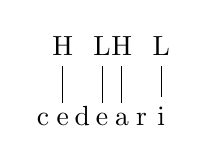
\begin{tikzpicture}
%tone tier (4 tones)
\node (t1) at (1.25,1) {H};
\node (t2) at (1.75,1) {L};
\node (t3) at (2,1) {H};
\node (t4) at (2.5,1) {L};
%segment tier (7 segments)
\node[anchor=base] (c1) at (1,0) {c} ;
\node[anchor=base] (v1) at (1.25,0) {e} ;
\node[anchor=base] (c2) at (1.5,0) {d} ;
\node[anchor=base] (v2) at (1.75,0) {e} ;
\node[anchor=base] (v3) at (2,0) {a} ;
\node[anchor=base] (c3) at (2.25,0) {r} ;
\node[anchor=base] (v4) at (2.5,0) {i} ;
%association lines (4)
\draw (t1) -- (v1);
\draw (t2) -- (v2);
\draw (t3) -- (v3);
\draw (t4) -- (v4);
\end{tikzpicture}
\z

\noindent It's recommended that you play around with spacing and node placement here. Similar to the procedure laid out in \sectref{sec:diercks:PhonDia}, we like to start by anchoring the segments themselves and subsequently placing the tones to match the x values for their corresponding vowels. Note that one advantage of using the \texttt{TikZ} package for autosegmental diagrams is the ease with which you can control your association lines. For example, let's say we have a Syncope rule that deletes the second /e/ from the underlying form above, leaving its `L' tone unassociated. We simply \textbf{delete or comment out the /e/ node} as well as \textbf{its tonal association line}:

\ea Tonal associations for /cedari/ after Syncope applies

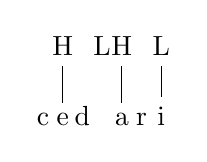
\begin{tikzpicture}
%tone tier (4 tones)
\node (t1) at (1.25,1) {H};
\node (t2) at (1.75,1) {L};
\node (t3) at (2,1) {H};
\node (t4) at (2.5,1) {L};
%segment tier (now only 6 segments)
\node[anchor=base] (c1) at (1,0) {c} ;
\node[anchor=base] (v1) at (1.25,0) {e} ;
\node[anchor=base] (c2) at (1.5,0) {d} ;
\node[anchor=base] (v3) at (2,0) {a} ;
\node[anchor=base] (c3) at (2.25,0) {r} ;
\node[anchor=base] (v4) at (2.5,0) {i} ;
%association lines (now only 3 lines)
\draw (t1) -- (v1);
\draw (t3) -- (v3);
\draw (t4) -- (v4);
\end{tikzpicture}
\z

\noindent Now imagine that, after Syncope applies, a Reassociation rule associates stray tones with the following vowel. We can show the reassociation of `L' by connecting it to the [a] segment:

\ea Tonal associations for /cedari/ after Syncope and Reassociation

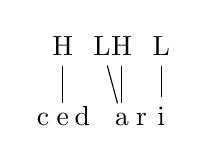
\begin{tikzpicture}
%tone tier 
\node (t1) at (1.25,1) {H};
\node (t2) at (1.75,1) {L};
\node (t3) at (2,1) {H};
\node (t4) at (2.5,1) {L};
%segment tier
\node[anchor=base] (c1) at (1,0) {c} ;
\node[anchor=base] (v1) at (1.25,0) {e} ;
\node[anchor=base] (c2) at (1.5,0) {d} ;
\node[anchor=base] (v3) at (2,0) {a} ;
\node[anchor=base] (c3) at (2.25,0) {r} ;
\node[anchor=base] (v4) at (2.5,0) {i} ;
%association lines (back to 4)
\draw (t1) -- (v1);
\draw (t2) -- (v3);
\draw (t3) -- (v3);
\draw (t4) -- (v4);
\end{tikzpicture}
\z

\subsection{Tableaux}
While you can certainly make beautiful Optimality-Theoretic tableaux in the \texttt{tabular} environment, the \texttt{ot-tableau} package makes this task a little bit easier. The \texttt{ot-tableau} package uses the \texttt{tableau} environment, which functions similarly to the \texttt{tabular} environment. Here's a simple tableau with three candidates and three constraints with a known ranking, as indicated by the solid vertical lines between constraints:

\ea Simple tableau with known constraint ranking

\begin{tableau}{c|c|c} 
\inp{\ips{stap}} 
\const{*Complex} 
\const{Anchor-IO} 
\const{Contiguity-IO}
\cand{stap} \vio{*!} \vio{} \vio{} 
\cand[\Optimal]{sap} \vio{} \vio{} \vio{*}
\cand{tap} \vio{} \vio{*!} \vio{}
\end{tableau}
\z

%A few things to note here: 
    % 1. In the parameter in the first line of code, the `c's mean `constraint', not `center align'.
    %2. The input line is specified using the \inp command, and within that, the \ips command is used to render the text using TIPA and put it within slashes. If you don't want it to do this automatically, just get rid of the \ips command and add your slashes and IPA text manually.
    %3. The \Optimal command gives you the pointy finger.

Here's the same tableau, but with a dotted line separating the first and second constraints to indicate that the ranking relationship between these two constraints is unknown:

\ea Simple tableau with partially-known constraint ranking

\begin{tableau}{c:c|c}
\inp{\ips{stap}} 
\const{*Complex} 
\const{Anchor-IO} 
\const{Contiguity-IO} 
\cand{stap} \vio{*!} \vio{} \vio{} 
\cand[\Optimal]{sap} \vio{} \vio{} \vio{*} 
\cand{tap} \vio{} \vio{*!} \vio{}
\end{tableau}
\z

Finally, here's an example of a tableau where the incorrect constraint ranking gives us the wrong ``winner". The \bomb{} marks the candidate that wins (but shouldn't), and the \grimace{} marks the candidate that should win (but doesn't):

\ea Simple tableau with incorrect constraint ranking

\ShadingOn
\begin{tableau}{c|c|c}
\inp{\ips{stap}} 
\const{*Complex} 
\const{Contiguity-IO} 
\const{Anchor-IO} 
\cand{stap} \vio{*!} \vio{} \vio{} 
\cand[\grimace]{sap} \vio{} \vio{*!} \vio{} 
\cand[\bomb]{tap} \vio{} \vio{} \vio{*}
\end{tableau}
\z

\section{Conclusion}

Our Quick Reference Guide is quite long! Ah the irony. But we hope it helps you find your way around formatting of ACAL Proceedings papers. There are a host of relevant resources online, and if you hit a confusing puzzle you can almost always google ``my problem latex'' and find relevant articles on Stackexchange and other similar sites. This guide is not meant to be comprehensive at all, but rather is meant to introduce novices to the central issues necessary to write a paper for the ACAL Proceedings. If you have questions, please feel free to contact the ACAL \LaTeX{} committee at \href{mailto:acal.latex@gmail.com}{acal.latex@gmail.com}.

Thank you for your efforts to keep our proceedings Open Access with Language Science Press! 

\section*{Abbreviations}

It is a required part of volumes with Language Science Press that an abbreviations list be included, so you cannot omit this section.

\section*{Acknowledgements}

Paper acknowledgements must be listed here, not in a footnote in the paper. This \href{https://www.overleaf.com/latex/templates/acal-proceedings-latex-quick-reference-guide/fncrcrtgnxhv}{Quick Reference Guide} and the \href{https://www.overleaf.com/latex/templates/acal-proceedings-template/kxmngmsjvfqq}{corresponding Paper Template} borrow directly (with permission) from corresponding documents written by Michael Diercks and Franny Brogan for linguistics students at Pomona College. Diercks' original \LaTeX{} teaching materials were created with assistance from Claire Halpert, Nico Baier, Jason Zentz, Maddy Bossi, and Mica Clausen. Our gratitude to the ACAL \LaTeX{} committee for their input to this template (especially Peter Jenks, Ken Steimel, and Matthew Faytak). 

\sloppy %this command eliminates a quirk that appears in the bibliography, you can just leave it here.
\printbibliography[heading=subbibliography,notkeyword=this]

\end{document}

%To be added to the ACAL \LaTeX{} template, someday: glossing with leipzig, advanced instructions for arrows
